\documentclass[11pt]{article}
\usepackage{amsmath}
\usepackage{graphicx}
\usepackage{listings}
\usepackage{color}
\usepackage{setspace}
\usepackage[english]{babel}
\usepackage[utf8]{inputenc}
\usepackage{fancyhdr}
\usepackage[margin=1in,footskip=0.25in]{geometry}
\pagestyle{fancy}



\definecolor{Code}{rgb}{0,0,0}
\definecolor{Decorators}{rgb}{0.5,0.5,0.5}
\definecolor{Numbers}{rgb}{0.5,0,0}
\definecolor{MatchingBrackets}{rgb}{0.25,0.5,0.5}
\definecolor{Keywords}{rgb}{0,0,1}
\definecolor{self}{rgb}{0,0,0}
\definecolor{Strings}{rgb}{0,0.63,0}
\definecolor{Comments}{rgb}{0,0.63,1}
\definecolor{Backquotes}{rgb}{0,0,0}
\definecolor{Classname}{rgb}{0,0,0}
\definecolor{FunctionName}{rgb}{0,0,0}
\definecolor{Operators}{rgb}{0,0,0}
\definecolor{Background}{rgb}{0.98,0.98,0.98}

\lstnewenvironment{python}[1][]{
\lstset{
numbers=left,
numberstyle=\footnotesize,
numbersep=1em,
xleftmargin=1em,
framextopmargin=2em,
framexbottommargin=2em,
showspaces=false,
showtabs=false,
showstringspaces=false,
frame=l,
tabsize=4,
% Basic
basicstyle=\ttfamily\small\setstretch{1},
backgroundcolor=\color{Background},
language=Python,
% Comments
commentstyle=\color{Comments}\slshape,
% Strings
stringstyle=\color{Strings},
morecomment=[s][\color{Strings}]{"""}{"""},
morecomment=[s][\color{Strings}]{'''}{'''},
% keywords
morekeywords={import,from,class,def,for,while,if,is,in,elif,else,not,and,or,print,break,continue,return,True,False,None,access,as,,del,except,exec,finally,global,import,lambda,pass,print,raise,try,assert},
keywordstyle={\color{Keywords}\bfseries},
% additional keywords
morekeywords={[2]@invariant},
keywordstyle={[2]\color{Decorators}\slshape},
emph={self},
emphstyle={\color{self}\slshape},
%
}}{}


\renewcommand{\thesubsection}{\thesection.\alph{subsection}}
\usepackage{textcomp}
\usepackage{amsfonts}
\usepackage{amssymb}
\usepackage{bbm}
\usepackage{amsmath,amssymb,amsthm,enumitem}
\newtheorem{theorem}{Theorem}[section]
\newcommand\numberthis{\addtocounter{equation}{1}\tag{\theequation}}
\theoremstyle{definition}
\usepackage{amsmath}
\usepackage[]{algorithm2e}
\usepackage[noend]{algpseudocode}
\makeatletter
\def\BState{\State\hskip-\ALG@thistlm}
\makeatother
\newtheorem{definition}{Definition}[section]
\newcommand{\Var}{\mathrm{Var}}
\newtheorem{corollary}{Corollary}[theorem]
\DeclareMathOperator*{\E}{\mathbb{E}}
\newcommand*{\Scale}[2][4]{\scalebox{#1}{$#2$}}
\begin{document}
\rhead{Normal-Uniform Noise Model}


\section{The Expectation Maximization Algorithm}
There are many probabilistic models that do not have a closed form solution for the MLE and thus require a numerical algorithm. One such model is a mixture model and one such numerical algorithm is the Expectation Maximization Algorithm.  And in our case for defining the center of DNAse I or H3K27ac or whatever, we are looking at a model where the normal distribution defines \textit{signal} and the uniform distribution defines \textit{noise}. Our goal is to define the center of signal($\mu$), the spread of signal($\sigma^2$), and the proporprotion of signal to noise ($\pi$).  Our data will be a list of genomic coordinates within some start and stop range in the genome (probably MACs calls). 

\subsection{Mixture Models} 
Imagine for a second that you were presented data that looked liked this

\begin{figure}[!h]
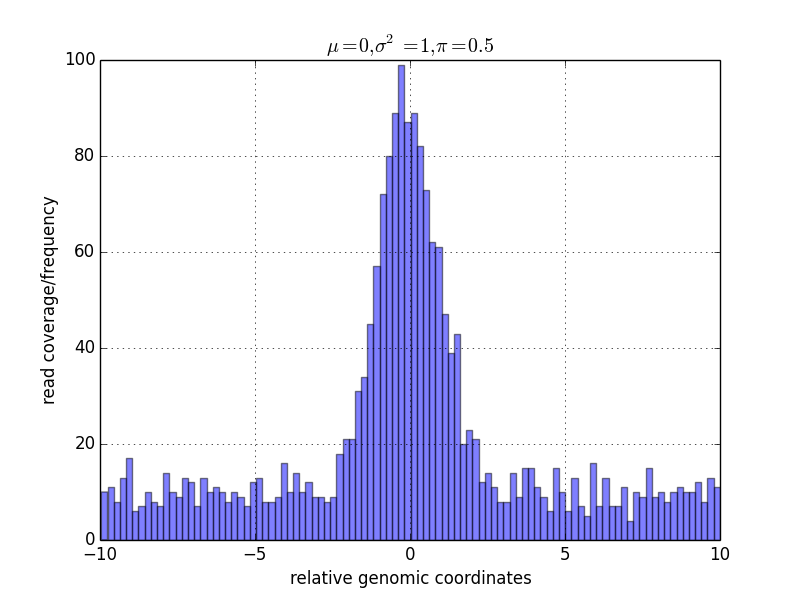
\includegraphics[scale=0.5]{NU_EXAMPLE}
\caption{MLE Estimators for $\mu$ and $\sigma^2$ will be complete thrown off by the presence of uniform noise. (kinda looks like ChIP data right?)}
\end{figure}
The above histogram was generated from this very simple mixture model


\begin{equation}
p(x|\Theta) = \pi\cdot f(x; \mu, \sigma^2) + (1-\pi)\cdot g(x; a,b)
\end{equation}
Here 
\begin{equation}
f(x|\mu_k,\sigma_k) = \frac{1}{\sqrt{2\pi\sigma_k^2}}e^{-\frac{(x-\mu_k)^2}{2\sigma_k^2}}
\end{equation}
and 
\begin{equation}
g(x|a,b) = \frac{1}{b-a}\cdot I(a\geq x \leq b)
\end{equation}

In short, a closed form analytic solution for the MLE of this model does not exist. To convince yourself look at the below likelihood function and attempt the MLE methodology. 
\begin{equation}
L(\Theta) = \prod_{i=1}^N \sum_{k=1}^M \pi_k p(x_i; \mu_k, \sigma_k)
\end{equation}
So what can we do? Well, the EM algorithm (developed by Rubiner in the 70's) is the most widely used algorithm for a latent variable model (here our latent variables are the component IDs for each data point). For a moment lets just assume we knew for each data point $x_i$ the associated component ID $k_i$, where lets just say $k_i=1$ if $x_i$ was generated from normal distribution and $k_i=2$ if $x_i$ was generated from the uniform distribution. Call $X=\{x_1, x_2, ..., x_n\}$ and $K=\{k_1,k_2, ... , k_n\}$ and so the complete data would $D=\{X, K\}$; take a moment to convince yourself that you could now easily find an MLE solution for each component with this knowledge. Thusly we can now define the complete data log likelihood. 

\begin{equation}
\log L(\Theta|X, K) = \sum_{i=1}^N\log{\pi_{k_i} p_{k_i}(x_i|\mu_{k_i}, \sigma^2_{k_i})}
\end{equation}
\noindent
The problem is of course that we don't know $K$ but if we treat $K$ as a random variable we can move forward. 
\subsection{Outline of the EM Algorithm}
The section following this one proves the correctness of the EM algorithm. However the below discussion will (hopefully) be enough for you to implement the algorithm. The EM algorithm alternates between two steps: (1. E-step) Compute the expectation of what we don't know $K$ given what we do know $X$ and then (2. M-step) maximize this conditional expectation. First we define the conditional expectation below,
\begin{equation}
Q(\Theta,\Theta^{t-1})=E[p(X,K|\Theta)|X, \Theta^{t-1}] = \sum_{k\in K}\log p(X,K| \Theta)\cdot p(K|X, \Theta^{t-1})\\
\end{equation}
where t is the iteration step in the EM loop. Here, the Q function can be defined thusly (I will leave it to you to prove...if you want...the correctness of this result).
\begin{equation}
Q(\Theta,\Theta^{t-1})=\sum_{k=1}^2\sum_{i=1}^N\log\pi_kp(k|x_i; \Theta^{t-1}) + \sum_{k=1}^2\sum_{i=1}^N\log p(x_i|\Theta^t) p(k|x_i; \Theta^{t-1})
\end{equation}
where we define 
\begin{equation}
\begin{split}
&p(k=1|x_i;\Theta^{t-1}) = \frac{ \pi\cdot f(x_i ;\Theta_l^{t-1}) }{ \pi\cdot f(x_i ;\Theta_l^{t-1}) + (1-\pi)\cdot g(x_i|l;\Theta_l^{t-1}) } \\
&p(k=2|x_i;\Theta^{t-1}) = \frac{   (1-\pi)\cdot g(x_i|l;\Theta_l^{t-1}) }{ \pi\cdot f(x_i ;\Theta_l^{t-1}) + (1-\pi)\cdot g(x_i|l;\Theta_l^{t-1}) } \\
\end{split}
\end{equation}
This completes the E-step. Now we only need to maximize the above expression, $Q(\Theta, \Theta^{t-1})$ with respect to all the parameters. We do this by differentiating $Q(\Theta, \Theta^{t-1})$ with respect to each parameter $\{\mu^t, \sigma^t , \pi^t \}$ and setting them equal to zero. I will leave you to verify that these expressions are correct. 
\begin{align}
\mu &:=\frac{1}{r_k}\cdot\sum_{i=1}^Nx_i\cdot r_i^k   \\
\sigma^2 &:=\frac{1}{r_k}\cdot\sum_{i=1}^N(x_i-\mu_k)^2\cdot r_i^k     \\
\pi &:= \frac{r_1}{r_1 + r_2}  
\end{align}
where $r_i^k = p(k|x_i;\Theta^{t-1})$ and $r_k = \sum_{i=1}^Nr_i^k$. 
\\
\\
\noindent
So this should be a fairly remarkable result! What this is saying is that for each iteration in the EM loop we take the weighted sample mean and weighted sample variance of each data point to the given component! This is guaranteed to converge and increase the log-likelihood at each iteration! The pseudo-code is given below. 

\begin{algorithm}[!h]
 \caption{The EM Algorithm for GMM}
 \KwData{$\{x_1, x_2, ... , x_n \}$}
 \KwResult{ $\Theta = \{\mu_1, \sigma_1, \pi_1,...,\mu_k, \sigma_k, \pi_k\}$ }
 initialization, note that you have set a specified number of mixtures/components to consider ($M$)\;
 initialization, randomly pick $\Theta$ with the correct dimension $M$\;
 
 \While{not converged}{
  E-Step\;
  \For{i=1 to N}{
 \begin{align*}
r_i^{k=1} = \frac{ \pi\cdot f(x_i ;\Theta_l^{t-1}) }{ \pi\cdot f(x_i ;\Theta_l^{t-1}) + (1-\pi)\cdot g(x_i|l;\Theta_l^{t-1}) } \\
r_i^{k=2} = \frac{   (1-\pi)\cdot g(x_i|l;\Theta_l^{t-1}) }{ \pi\cdot f(x_i ;\Theta_l^{t-1}) + (1-\pi)\cdot g(x_i|l;\Theta_l^{t-1}) } \\
\end{align*}
}
  M-Step\;
  \begin{align*}
\mu^t&:=\frac{1}{r_k}\cdot\sum_{i=1}^Nx_i\cdot r_i^{k=1}   \\
\sigma^{2,t} &:=\frac{1}{r_k}\cdot\sum_{i=1}^N(x_i-\mu_k)^2\cdot r_i^{k=1}     \\
\pi^t&:= \frac{r_{k=1}}{\sum_1^2 r_l}  
\end{align*}
Compute $L(\Theta^{t}) = \sum_{k=1}^M r_k$ \; 	
  
  \eIf{$L(\Theta^{t-1})-L(\Theta^{t})\leq 10^{-4}$  }
  {
   converged=True;
   }{
   converged=False;
  }
 }
\end{algorithm}

Real quick: This is the most important tip I can give when running the EM on read coverage data. We have for each genomic position a coverage value. Lets say for position 10,000 on chromosome 1 there where 1,000 reads. The naive solution to EM algorithm would be to make a list and repeat genomic position 1,000 times and run the EM. This of course is really really slow. A better way is to just calculate $r_i^k$ for that position and then mutliply by 1,000 sense we know this value won't change for the other 9,999 replicates. You just need to make sure you are keeping track of the proper normalizations when you do this, but its way way faster to do mutltiplication then do a for loop for 1,000 and calculated the same normal/uniform distribution over and over again. 


\subsection{Proof of the EM}
I want to provide a brief sketch to the proof of the EM algorithm (I came across this approach a couple months ago and I feel its more intuitive than other proofs of this algorithm).  I recognize this might seem really hard, so don't feel bad if this doesn't make sense. But at the very least try to work your way through it. 
\\
\\
\noindent
Lets start by defining the incomplete data likelihood, in terms of the complete data likelihood. We note, $p(x) = \sum_{y\in Y} p(x,y)$ (this is the definition of a marginal distribution...really all we are doing is summing away the things we don't care about,i.e. Y). 

\begin{equation}
p(X|\Theta) = \sum_{k\in K}p(X,K|\Theta)
\end{equation}
Again, we note that the direct optimization of $p(X|\Theta)$ is really hard, but the optimization of $p(X,K|\Theta)$ is really easy. Thusly we define a distribution over the latent variables $q(K)$ and note that the following decomposition holds.

\begin{equation}
\log p(X|\Theta) = \mathcal{L}(q,\theta) + KL(q||p)
\end{equation}
where we have defined 
\begin{equation}
\mathcal{L}(q,\theta) = \sum_kq(k)\log\frac{p(X,K|\theta)}{q(k)} ;
KL(q||p) 	= -\sum_k q(k)\log\frac{p(K|X, \theta)}{q(k)}
\end{equation}
$\mathcal{L}$ is whats called a functional (its a function that takes in a function! ). So far we have not specified the form of $q(K)$ just that it is a valid probability distribution (i.e. $\sum_kq(K) = 1$).
Now lets really dive into how we got this decomposition (most books do not do this...I don't know why...they just present that decomposition and move forward...so count yourself lucky!). Really this proof is just about multiplying by 1!
\begin{align}
p(X;\Theta)&= \sum_{k\in K}q(K)p(X;\Theta)\\
\log p(X;\Theta) &=\sum_{k\in K}q(K)\log\Big(p(X;\Theta)\Big)\\
&= \sum_{k\in K}q(K)\log\Big(p(K|X;\Theta)p(X;\Theta)\frac{1}{p(K|X;\Theta)}\Big)  \mbox{...multiply by $\frac{p(K|X)}{p(K|X)}$}\\  
&= \sum_{k\in K}q(K)\log\Big(p(X;\Theta)p(K|X;\Theta)\frac{1}{p(K|X;\Theta)} q(K)\frac{1}{q(K)}\Big)  \  \mbox{...multiply by $\frac{q(K)}{q(K)}$}\\  
&= \sum_{k\in K}q(K)\log\frac{p(X,K;\Theta)}{q(K)} + \sum_{k\in K}q(K)\log\frac{q(K)}{p(K|X;\Theta)} \\  
&= \sum_{k\in K}q(K)\log\frac{p(X,K;\Theta)}{q(K)} - \sum_{k\in K}q(K)\log\frac{p(K|X;\Theta)}{q(K)}  
\end{align}
Let's take a breather for a second and appreciate the last equation and what it says. Somehow (by multiplying by 1!) we have recovered the complete data log likelihood function (first term) and the KL divergence of q and p (the second term). Without proof, although the proof is quite intuitive as well, we say the KL diverge is always non-negative and zero if q and p are exactly the same. It is worth noting however that although this seems like a distance metric, it is not reflective i.e. ($KL(q||p) \neq KL(p||q)$). We can visualize the above decomposition with the below figure. 


\begin{figure}[!h]
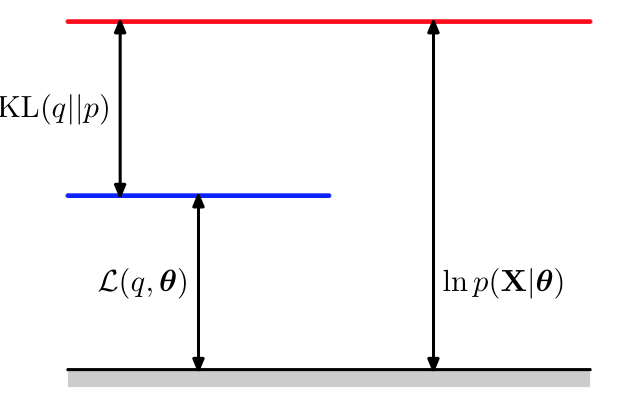
\includegraphics[scale=0.5]{KL}
\caption{Sense the KL divergence is always non-negative, $\mathcal{L}$ provides a lower bound on the incomplete data log-likelihood. Thus maximizing that lower bound will always give us a better estimate for the latent variables/parameters.}
\end{figure}
So now the question becomes what is a good equation for $q$. We know that if we set $q=p(Z|K, \Theta)$ than this would give us the exact distribution for $\log p(X|\Theta)$ however that doesn't really help us sense we don't know $\Theta$ and can't maximize however, if we set $q=p(Z|K,\Theta^{old})$ or $q=p(Z|K,\Theta^{t-1})$, then conditional probability of what we don't know given what we do know, then it seems like we can proceed, sense we only need to maximize $\mathcal{L}$ with respect to $\Theta$ (not $\Theta^{old}$), to increase this lower bound. So if we insert $q=p(Z|K,\Theta^{old})$ into the last equation from above we get, 
\begin{align}
p(X;\Theta)&=\sum_{k\in K}p(Z|K,\Theta^{old})\log\frac{p(X,K;\Theta)}{p(Z|K,\Theta^{old})} - \sum_{k\in K}p(Z|K,\Theta^{old})\log\frac{p(K|X;\Theta)}{p(Z|K,\Theta^{old})} \\
&=\sum_{k\in K}p(Z|K,\Theta^{old})\log{p(X,K;\Theta)}-\sum_{k\in K}p(Z|K,\Theta^{old}){p(Z|K,\Theta^{old})} - KL(q||p)\\
&=Q(\Theta, \Theta^{old}) + const.
\end{align}
where const. is just the negative entropy of q and the KL divergence of q and p. The negative entropy doesn't concern $\Theta$ so we don't need to consider it in our maximization step and sense the KL divergence, again is always positive we only care about maximizing the lower bound $Q(\Theta, \Theta^{old})$. So this is great! We have proved that our EM is an iterative process that will always increase the incomplete log-likelihood! 

























\end{document}
